\chapter{Anhang: Implementierung}
\section{Beispiel: Ergebnisse im Quellverzeichnis}
\label{attachement:python:results}
In Abbildung~\ref{fig:source_folder} ist das Quellverzeichnis dargestellt.
Es beinhaltet die Quelldateien, die analysiert werden sollen.
\begin{figure}[H]
	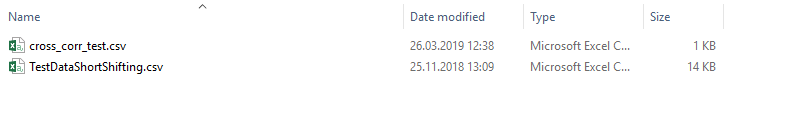
\includegraphics[width=\linewidth]{attachements/python/source_folder.PNG}
	\caption[Anhang: Quellverzeichnis vor der Ausführung]{Abbildung des Quellverzeichnisses, bevor das Skript ausgeführt wurde\footnotemark.}
	\label{fig:source_folder}
\end{figure}
\footnotetext{Quelle: Eigene Darstellung}

Bei der Ausführung des Skripts werden die generierten PDF-Dateien im Quellverzeichnis mit abgelegt.
Dadurch ergibt sich danach das in Abbildung~\ref{fig:source_folder_results} dargestellte Ergebnis.
\begin{figure}[H]
	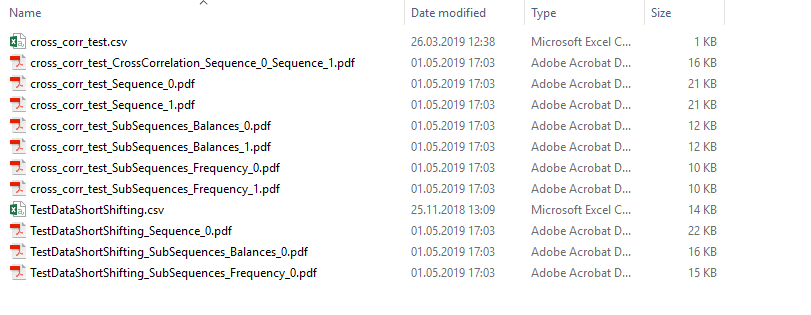
\includegraphics[width=\linewidth]{attachements/python/source_folder_result.PNG}
	\caption[Anhang: Quellverzeichnis nach der Ausführung]{Abbildung des Quellverzeichnisses, nachdem das Skript ausgeführt wurde\footnotemark.}
	\label{fig:source_folder_results}
\end{figure}
\footnotetext{Quelle: Eigene Darstellung}

\section{Log-Meldungen des automatisierten Skripts}
\label{attachement:python:log}
Das automatisierte Skript schreibt diverse Log-Meldungen in die Konsole.
Listing~\ref{lst:pythonlogs} ist ein Beispiel dafür, was durch das Skript geloggt wird.

\lstnewenvironment{PythonLogs}
{\lstset{
		captionpos=b,
		frame=single,
		label={lst:pythonlogs},
		caption={Anhang: Beispiel für generierte Log-Meldungen},
		showspaces=false,
		showtabs=false,
		breaklines=true,
		showstringspaces=false,
		breakatwhitespace=true,
		escapeinside={(*@}{@*)},
		commentstyle=\color{greencomments},
		morecomment = [l]{\#\ },
		morekeywords={ },
		keywordstyle=\color{blue},
		stringstyle=\color{black},
		morestring=[b]",
		basicstyle=\ttfamily\footnotesize,
		numberbychapter=false}}{}

\begin{PythonLogs}
Reading files from source path:
.\sourceFiles
Found 2 source files

Reading data from  .\sourceFiles\cross_corr_test.csv ...
Found sequences:  2
Expanding data for .\sourceFiles\cross_corr_test.csv Sequence 0
Expanding data for .\sourceFiles\cross_corr_test.csv Sequence 1

Reading data from  .\sourceFiles\TestDataShortShifting.csv ...
Found sequences:  1
Expanding data for .\sourceFiles\TestDataShortShifting.csv Sequence 0

Calculating frequency for .\sourceFiles\cross_corr_test.csv Sequence 0
Calculating frequency for .\sourceFiles\cross_corr_test.csv Sequence 1
Calculating balance for .\sourceFiles\cross_corr_test.csv Sequence 0
Calculating balance for .\sourceFiles\cross_corr_test.csv Sequence 1
Calculating block size information for .\sourceFiles\cross_corr_test.csv
Calculating block infos for .\sourceFiles\cross_corr_test.csv Sequence 0
Calculating block infos for .\sourceFiles\cross_corr_test.csv Sequence 1

Calculating frequency for .\sourceFiles\TestDataShortShifting.csv Sequence 0
Calculating balance for .\sourceFiles\TestDataShortShifting.csv Sequence 0
Calculating block size information for .\sourceFiles\TestDataShortShifting.csv
Calculating block infos for .\sourceFiles\TestDataShortShifting.csv Sequence 0

Generating pdfs...
Generating pdf reports for .\sourceFiles\cross_corr_test.csv Sequence 0
Generating pdf reports for .\sourceFiles\cross_corr_test.csv Sequence 1
Generating pdf reports for .\sourceFiles\TestDataShortShifting.csv Sequence 0

Crosscorrelation for file .\sourceFiles\cross_corr_test.csv
.\sourceFiles\cross_corr_test.csv exporting Cross-Correlation between sequence 0 and 1
\end{PythonLogs}


\section{Verwendung von Docker}
\label{docker:examples}

Ein verwendbarer Docker-File ist im Quellverzeichnis als \enquote{dockerfile} abgelegt.
Aus dieser Datei kann ein Image erstellt werden, dass Python und die notwendigen Bibliotheken enthält.
Aus diesem Image kann ein Container erstellt werden, in dem ein Quellverzeichnis des Host-Rechners gemountet wird.
Dadurch hat der Container Zugriff auf die Dateien in diesem Ordner und kann diese Verarbeiten.
Im Folgenden sind die notwendigen Befehle dokumentiert, um das Image und den Container zu erstellen und zu verwenden.
\lstset{literate=%
	{Ö}{{\"O}}1
	{Ä}{{\"A}}1
	{Ü}{{\"U}}1
	{ß}{{\ss}}1
	{ü}{{\"u}}1
	{ä}{{\"a}}1
	{ö}{{\"o}}1
	{~}{{\textasciitilde}}1
}
\lstnewenvironment{DockerCommands}
{\lstset{
		captionpos=b,
		frame=single,
		label={lst:pythonlogs},
		caption={Anhang: Beispiel für die Verwendung von Docker},
		showspaces=false,
		showtabs=false,
		breaklines=true,
		showstringspaces=false,
		breakatwhitespace=true,
		escapeinside={(*@}{@*)},
		commentstyle=\color{greencomments},
		morecomment = [l]{\#\ },
		morekeywords={ },
		keywordstyle=\color{blue},
		stringstyle=\color{black},
		morestring=[b]",
		basicstyle=\ttfamily\footnotesize,
		numberbychapter=false}}{}
	
\begin{DockerCommands}
Befehlstemplate zur Erstellung des Images. Der Name füur das Image ist frei wählbar, muss aber in den folgenden Befehlen verwendet werden:
	docker build . -t <image_name>
Beispiel:
		docker build . -t analysisImage
Die Skripte die verwendet werden, sind ein fester Bestandteil des Images. Wenn Änderungen an den Skripten vorgenommen werden, muss auch das Image neu erstellt werden.
Folglich muss dann auch der Container neu erstellt werden.
		
Befehlstemplate zur Erstellung eines Containers:
	docker create  -v <Pfad zum Quellordner>:/usr/src/app/sourceFiles  --name <container_name>  <image_name>
Beispiel:	
	docker create  -v C:\Temp\sourcefiles:/usr/src/app/sourceFiles  --name MyAnalysisContainer  analysisImage
Der Pfad zum Quellordner ist ein fester Bestandteil des Containers und kann nicht ohne weiteres verändert werden.
Soll ein anderer Ordner verwendet werden, muss ein neuer Container erzeugt werden. Dadurch ist auch die Möglichkeit gegeben, unterschiedliche Ordner in unterschiedlichen Containern zu verwenden.

Befehlstemplate zur Ausführung eines Containers:
	docker start -a <container_name>
Beispiel:
	docker start -a MyAnalysisContainer
Dadurch wird ein Container ausgeführt und die Ausgabe wird auf der Konsole ausgegeben. Der Container beendet sich nach Ausführung von selbst.

Weitere, hilfreiche Befehle:

Löschen eines Containers:
	docker rm <container_name>
Beenden eines Containers:
	docker stop <container_name
Löschen eines Images:
	docker rmi <image_name>
\end{DockerCommands}